\chapter{Preliminary concepts}

\label{ch:preliminary}

\section{Dynamical Systems}

% [introducir bien el tema]. 

The general form for a finite-dimensional dynamical system is the following.

\begin{equation}
    \dfrac{d\bm{u}}{dt} = \bm{f}(\bm{u}, \eta), \qquad \bm{f} : \mathbb{R}^N \times \mathbb{R}^{n_\eta} \to \mathbb{R}^N.
    \label{eq:def_ds}
\end{equation}

Here, $\bm{u}$ represents the state vector of the system, it might correspond to the
concentrations of different chemicals, the population of certain species or the amplitude
of an electric field. The temporal evolution of the state of the system is thus determined by 
the vector function $\bm{f}$. This function may, in turn, depend on one or more control
parameters $\eta$ relevant to the modeled experiment (i.e. driving frequency, pumping power, etc.).
Extensions of the above formulation can be envisaged, mainly in the form of partial differential equations
or even integro-differential equations describing infinite dimensional systems. For the sake of simplicity,
only finite-dimensional systems will be relevant for the following discussion.

In this thesis, different dynamical systems in the form of Eq.~(\ref{eq:def_ds}) with a {\em nonlinear} function
$\bm{f}$ will be considered. Although it might be argued that, at a fundamental level, the physical laws
that describe the evolution of a system are linear (such as the Schrödinger equation), when one looks at meso- or macroscopical
systems, nonlinear terms naturally arise due to the coarse-graining of the microscopical degrees of freedom~\cite{kardar2007statistical}.


In the case of a nonlinear dynamical system, it becomes extremely difficult, and often impossible, to find
general explicit solutions of Eq.~(\ref{eq:def_ds}). But it turns out that in most cases, an in-depth
description of the model can be provided by studying only the steady states ($\bm{f}(\bm{u}, \eta) = 0$) and their qualitative changes as parameters 
are varied. In other words, the problem can be reduced to finding the {\em equilibria} and {\em bifurcations} of the system.
In the following section, the elementary bifurcations a system can experience will be described.

\section{Bifurcations}

One of the pioneers in identifying the importance of bifurcations in the study of dynamical systems
was Henri Poincaré while studying the different stable
configurations of a gravitating rotating fluid, along with their respective stability~\cite{poincare1885equilibre}. 
In doing so, he coined the
term {\em bifurcation}, refering to the point in the parameter space at which different solutions branch off from another solution.
To this day, his definition remains valid and, more formally, corresponds to a qualitative change 
in the system's behavior, related to the transition between different equilibria or to the exchange of stability,
as a control parameter is varied~\cite{strogatz2018nonlinear}.


% Ideas:
% \begin{enumerate}
%     \item saddle-node for genes pp 249
%     \item magnetism Landau Pitchfork
%     \item Hopf, van der pol, bici
% \end{enumerate}

\subsection{Saddle-Node bifurcation}

{\em Saddle-node} or {\em fold} bifurcations provide the simplest mechanism 
for which a pair of stable and unstable equilibria can be created (or destroyed) 
as the control parameter is changed~\cite{strogatz2018nonlinear}. Although they 
arise in a huge variety of systems~\cite{Jackson_1989}, close to the bifurcation 
point, the dynamics can always be reduced to
the following minimal or {\em normal form}.

\begin{equation}
    \dfrac{du}{dt} = \eta - u^2
    \label{eq:pre_bif_sn}
\end{equation}

Following the notation of Eq.~(\ref{eq:def_ds}), u represents the state variable
and $\eta$ the control parameter. For $\eta > 0$, the system presents two equilibria $u_{\pm} = \pm\sqrt{\eta}$, where $u_+$ is
stable and $u_-$ unstable. An interesting case occurs when $\eta = 0$, at which point $u = 0$ is
half-stable (stable for positive perturbations and unstable for negative perturbations). Lastly,
for $\eta < 0$ there are no equilibria. Figure~(\ref{fig:pre_bifs_sn}) provides a visual representation
of the previous analysis.

In short, as the bifurcation parameter $\eta$ is decreased (increased)
starting from positive (negative) values, the two equilibria attract (repel) each other and suddenly annihilate (appear).

\begin{figure}[h]
    \centering
    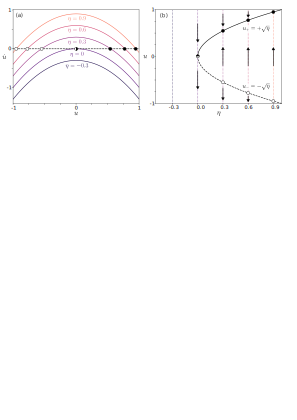
\includegraphics[width=\textwidth]{imagenes/framework/bif_sn_f.pdf}
    \caption{Prototipical scenario for a saddle-node bifurcation. (a) Phase space
    showing both stable and unstable fixed points for different values of $\eta$. 
    Black (white) circles represent
    stable (unstable) fixed points. (b) Bifurcation diagram showing
    the creation of a stable-unstable pair of fixed points. Solid (dashed) line represents
    stable (unstable) branch.}
    \label{fig:pre_bifs_sn}
\end{figure}

\begin{exmp}
    For centuries, the mystery of synchronization between fireflies has
    captivated the scientific community, and only recently has it been
    partially unveiled. Although the topic is intricate and will be discussed
    in more detail in Section~\ref{sec:phase_oscillators},
    we will aim to shed {\em light} on this topic only with the knowledge of saddle-node bifurcations
    and a simple model proposed by Ermentrout and Rinzel~\cite{ermentrout1984beyond}. 
    
    Consider the problem
    of a firefly flashing under the presence of a periodically flashing light.
    We will model the flashing of the firefly with an angular variable $\theta$
    such that $\theta = 0$ represents the firefly's flash. The firefly has its 
    own inherent frequency $\omega$, i.e. in the absence of stimuli 
    $\dot{\theta} = \omega$. On the other hand, the periodic stimulus will be
    represented by a phase $\phi$ that satisfies $\dot{\phi} = \Omega$, where 
    $\Omega$ is of course the stimuli period. In order to synchronize with the
    stimuli, the firefly will either want to speed up if it is lagging behind
    or slow down if it is going too fast. The simplest non-linear model that
    fulfills these assumptions is the following,
    \begin{align*}
        \dot{\phi} &= \Omega, \\
        \dot{\theta} &= \omega + A \sin(\phi -  \theta).
    \end{align*}

    Subtracting both equations and defining $\varphi = \dot{\phi} - \dot{\theta}$
    yields 

    \begin{equation*}
        \dot{\varphi} = \Omega - \omega - A \sin \varphi,
    \end{equation*}

    \noindent which can be adimensionalized by rescaling $t \to At$ and introducing
    the non-dimensional parameter $\mu = (\Omega - \omega)/A$,

    \begin{equation}
        \dot{\varphi} = \mu - \sin \varphi.
        \label{eq:pre_bif_sn_exmp}
    \end{equation}

    For $\mu = 0$ where the forcing and intrinsic frequencies are the same, there
    is a stable fixed point at $\varphi = 0$ and an unstable fixed point at $\varphi = \pi$.
    As $\mu$ increases, both equilibria approach each other until they collide for $\mu=\mu_c=1$
    at $\varphi = \pi/2$
    and then disappear for $\mu > 1$. We can recognize that the pair of fixed
    points appear (or disappear) through a saddle-node bifurcation.
    
    Moreover, close to the bifurcation point where $\mu_c = 1$ and $\varphi_c = \pi/2$,
    we can do a Taylor expansion: $\mu = 1 + \eta$ and $\varphi = \pi/2 + u$ 
    where $\eta, u \ll 1$. Using the identity $\sin \varphi = \sin (\pi/2 + u) = \cos u$
    and inserting the previous ansatz into Eq.~(\ref{eq:pre_bif_sn_exmp}) yields
    the following
    \begin{align*}
        \dot{\varphi} = \dot{u} &= 1 + \eta - \cos u, \\ 
        &\approx 1 + \eta - (1 - \dfrac12 u^2), \\
        &= \eta - \dfrac12 u^2,
    \end{align*}

    \noindent which after adequate rescaling corresponds exactly with the saddle-node
    normal form.
    

\end{exmp}

\subsection{Pitchfork bifurcation}

{\em Pitchfork} bifurcations typically arise in systems with reflection symmetry and 
provide a universal mechanism for symmetry-breaking~\cite{strogatz2018nonlinear}. 
A simple example is given by the statistical description of magnetization. 
In the absence of an external field, the net magnetization $m$ 
(below the critical temperature $T_c$) can either be positive or negative 
with no preferred orientation, thus depending only on the initial condition. On the
other hand, if the system is heated above the critical temperature, no net magnetization
is observed, i.e. $m=0$. In the context of statistical mechanics, this second-order
transition can be described by a mean-field approximation from Landau 
theory~\cite{landau2013statistical,kardar2007statistical}, where
the free energy functional is expanded in (even) powers of $m$, thus arriving at exactly
the pitchfork normal form, given by

\begin{equation}
    \dfrac{du}{dt} = \eta u - u ^ 3.
    \label{eq:pre_bif_pitchfork}
\end{equation}

As shown in Fig.~(\ref{fig:pre_bif_pitchfork}), for $\eta < 0$ there is only one 
equilibrium of Eq.~(\ref{eq:pre_bif_pitchfork}), it is stable and corresponds
to the trivial solution $u=0$. For $\eta > 0$, the trivial solution loses stability
and two stable symmetric branches $u_\pm = \pm \sqrt{\eta}$ emerge. 

\begin{figure}[h]
    \centering
    \includegraphics[width=\textwidth]{imagenes/framework/bif_pitch_f.pdf}
    \caption{Prototipical scenario for a pitchfork bifurcation. (a) Phase space
    showing both stable and unstable fixed points for different values of $\eta$. 
    Black circles represent stable fixed points, the grey circle represents a stable for $\eta < 0$
    and unstable for $\eta > 0$ fixed point. (b) Bifurcation diagram showing
    the emergence of two stable branches at the bifurcation, along with the change of
    stability of the trivial solution. Solid (dashed) lines represent
    stable (unstable) branches.}
    \label{fig:pre_bif_pitchfork}
\end{figure}

Two types of pitchfork bifurcations should be distinguished: the {\em supercritical} 
and the {\em subcritical} case. The former corresponds to Eq.~(\ref{eq:pre_bif_pitchfork})
and was discussed above. In the latter, the two symmetric branches that emerge at the bifurcation
point are unstable. In that case, the cubic term in the normal form has a positive sign and
a negative quintic term is added to ensure the solution is bounded, and thus, that is physically
relevant. The modified normal form corresponds to Eq.~(\ref{eq:pre_bif_pitchfork_subcritical}).

\begin{equation}
    \dfrac{du}{dt} = \eta u + u ^ 3 - u^5.
    \label{eq:pre_bif_pitchfork_subcritical}
\end{equation}

Moreover, due to the additional quintic term, the symmetric branches are stabilized 
at a secondary saddle-node bifurcation point $\eta_{sn}$, as shown
in Fig.~\ref{fig:pre_bif_subpitchfork}. It is important to mention that in subcritical
bifurcation, a hysteresis loop is typically observed. 
%For instance, Fig.~\ref{fig:pre_bif_subpitchfork}

\begin{figure}[h]
    \centering
    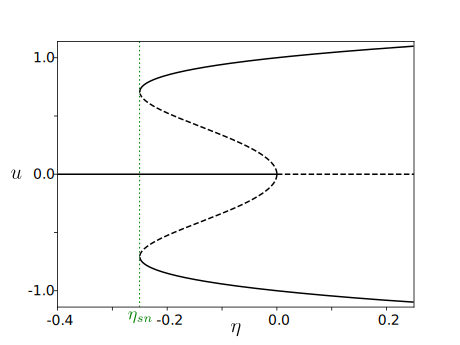
\includegraphics[width=0.6\textwidth]{imagenes/framework/bif_pitch_subcritical.pdf}
    \caption{Bifurcation diagram for the subcritical pitchfork. At the bifurcation point
    for $\eta=0$, two symmetric unstable branches emerge and gain stability after undergoing
    a saddle-node bifurcation for $\eta=\eta_{sn}=-\frac14$. The trivial solution is stable for $\eta < 0$
    and unstable for $\eta > 0$.}
    \label{fig:pre_bif_subpitchfork}
\end{figure}


\subsection{Andronov-Hopf bifurcation}

The two bifurcations discussed previously describe the emergence of steady states or fixed points. 
More specifically, they belong to the class of {\em stationary} bifurcations. Here, a different class of bifurcations will be introduced,
that of {\em dynamical} bifurcations, in which dynamical equilibria emerge. The simplest scenario is the Andronov-Hopf bifurcation
that allows for the emergence of a limit cycle or, in other words, a periodic equilibrium. Since oscillations are impossible in 
one dimension~\cite{strogatz2018nonlinear}, this bifurcation can only be present in systems of two or more dimensions. For simplicity, the following
analysis will be restricted to only two dimensions. Nevertheless, it can easily be extended to the more general case of arbitrary dimensions.
The normal form can be written in a compact form as a complex equation, Eq.~(\ref{eq:hopf}), for the
order parameter $A = x +iy$. It is important to mention that
the coefficient accompanying the cubic term could be complex, in that case, it corresponds to
the Stuart-Landau equation~\cite{landau1944problem,stuart1958non} which
is the homogeneous part of the widely known Complex Ginzgurg-Landau equation~\cite{aranson2002world}.

\begin{equation}
    \dfrac{dA}{dt} = (\eta + i\omega)A - |A|^2 A.
     \label{eq:hopf}
\end{equation}

It can directly be observed that there is a trivial fixed point at $A=0$. Linear stability analysis around this fixed point 
reveals a pair of complex eigenvalues $\lambda_\pm = \eta \pm i\omega$. Therefore, for $\eta < 0$ the fixed point is a stable
focus, whereas for $\eta > 0$, the eigenvalues have crossed the imaginary axis rendering the focus unstable. Moreover,
by rewriting Eq.~(\ref{eq:hopf}) in polar coordinates $A = re^{i\theta}$, the emergence of a limit cycle is evidenced.

\begin{align}
    \dot{r} &= r(\eta - r^2),\\
    \dot{\theta} &= \omega.
    \label{eq:hopf_polar}
\end{align}

From Eq.~(\ref{eq:hopf_polar}) it can be observed that a limit cycle emerges from $\eta=0$ with frequency $\omega$ and an 
amplitude $|A| = r = \sqrt{\eta}$ that increases continuously from zero. 
Similarly, as in the pitchfork bifurcation, this case corresponds to a supercritical
bifurcation given that the limit cycle arising from the bifurcation is stable. Furthermore, the two results mentioned previously
apply also in general, namely, that close to the
bifurcation point $\eta_c$, the amplitude of the limit cycle grows with $\sqrt{\eta - \eta_c}$ and the frequency is approximately
the imaginary part of the eigenvalue at the bifurcation point: $\operatorname{Im}{\lambda(\eta_c)}$.


\begin{figure}[h]
    \centering
    \includegraphics[width=0.8\textwidth]{imagenes/framework/hopf_phasespace.pdf}
    \caption{Phase plane trajectories of Eq.~(\ref{eq:hopf}) showing a stable
    focus for $\eta = -0.3$ in the left panel and a stable limit cycle for $\eta=0.3$
    in the right panel}
\end{figure}

There is, however, a subcritical variation
of the Andronov-Hopf bifurcation in which the emerging limit cycle is unstable and may stabilize at a secondary bifurcation point.
The normal form is similar to the subcritical pitchfork since the cubic term has now the opposite sign and a quintic term is added to ensure the solution is bounded.
Due to the additional quintic term, the emerging limit cycle stabilizes at $\eta_{sn} = -\frac14$ through
a saddle-node bifurcation.

\begin{equation}
    \dfrac{dA}{dt} = (\eta + i\omega) A + |A|^2 A - |A|^4A
\end{equation}

\begin{figure}[h]
    \centering
    \includegraphics[width=0.9\textwidth]{imagenes/framework/hopf_supersub.pdf}
    \caption{The subcritical and supercritical scenarios of the Andornov-Hopf
    bifurcation. Panel (a) shows the supercritical case and panel (b) shows the subcritical
    case.}
\end{figure}

\section{Localized Structures}
\label{sec:fra_LS}

In the previous section, the simplest mechanisms for the emergence and
change of stability of solutions have been discussed, yet little attention
has been devoted to the solutions themselves. Indeed, in nonlinear dynamical
systems, an enormous variety of equilibria are possible. In this section,
special attention will be paid to one particular kind class of equilibria,
the so-called localized structures. 

% Almost a century ago, our understanding of elementary or quantum particles went
% through a complete change of paradigm. Indeed, what was originally thought
% to be a microscopic speck of matter with a well-defined position, velocity and size
% was discovered instead to be a localized wave function lacking the former quantities.
% Half a century later, this change of paradigm carried over to meso- and macroscopical out-of-equilibrium
% systems. Nicolis and Prigogine~\cite{prigogine1977self} argued that the energy transfer present in these systems
% allows for complex and stable structures to form, such as localized structures. These localized states
% or particle-like solutions are supported by a robust balance between gains and losses and have been observed in a
% variety of systems due to their universality. 

\begin{figure}[h]
    \centering
    \includegraphics[width=0.7\textwidth]{imagenes/framework/LS/examples_ls.pdf}
    \caption{Examples of localized structures in nonlinear optics and granular media. Panels (a)-(d) show experimental observations of a drifting breather
    soliton in a microcavity~\cite{yi2018imaging}, a chaoticon in a liquid crystal light 
    valve~\cite{verschueren2013spatiotemporal}, an oscillon in a vibrating
    layer of sand~\cite{umbanhowar1996localized,aranson2006patterns}, and a three-dimensional
    light bullet in a waveguide array~\cite{minardi2010three}.}
    \label{fig:pre_ls_examplesls}
\end{figure}

Formally speaking, a LS corresponds to a well localized deviation of some reference background,
typically a homogeneous steady state, although it might also be periodic (in space) or oscillatory (in time).
As illustrated in Figure~(\ref{fig:pre_ls_examplesls}), they have been observed experimentally in one, two, and even three dimensions.
Their temporal dynamics are quite rich as well, they can present uniform motion, breathing or even chaotic behavior.
From a mathematical point of view, their description relies on partial differential equations or,
in the case of non-local systems, integro-differential equations. At least in one spatial dimension,
it is possible to think of LS as a homoclinic orbit asymptotically approaching the reference state
at the boundaries and performing an excursion in the neighborhood of another equilibrium in the center.
In the more general case of two and three-dimensional LSs, the picture becomes more complex but the
coexistence between two distinct equilibria remains necessary for the formation of LSs.


\subsection{Solitons}

Among localized states, a particularly interesting type are solitons. They were discovered
 for the first time in 1834 by John Scott Russell. He described them 
 as a {\em "large solitary [...] heap of water, which continued its course along the channel without change of form
or diminution of speed"} \cite{russell1845report}. These solitary waves were highly controversial
at the time until Korteweg and de Vries provided an integrable model for shallow water waves
and proved their existence in the now called Korteweg de Vries (KdV) equation \cite{korteweg1895xli}.
It was only a century later that the term soliton was coined by Zabusky and Kruskal
to emphasize their particle-like behavior after observing that solitons in the KdV equation could pass through each
other with no change in shape or speed \cite{zabusky1965interaction}. In the following
years, the newly discovered inverse scattering transform \cite{gardner1967method, gardner1974korteweg}
allowed to completely solve the KdV equation and find the analytical expression of solitons.
Immediately after, it was extended to other integrable and conservative equations such as the nonlinear Schrödinger (NLS)
equation \cite{shabat1972exact} and the sine-Gordon equation \cite{ablowitz1973method}. 
In these systems, they arise due to a balance between dispersion and nonlinearity. 


More recently, the term dissipative soliton (DS) was introduced to extend the previous definition
and refers to a qualitatively
similar state, but in driven dissipative systems, where there is a continuous energy influx and 
dissipation, requiring thus a balance between influx and dissipation. 
Although there is not a commonly agreed-upon definition of DSs, they typically
exhibit certain features. Firstly, DSs are attractors with well-defined amplitude and shape, and
possess a characteristic length independent of the system size or boundary. Moreover, they
tend to interact with other nearby DSs in a manner reminiscent of classical particles. 
As a result, they often receive the name of particle-like states. It is important to emphasize that classical (conservative) solitons and dissipative solitons
are two very different structures; the mathematics behind their presence, and therefore their
properties, are distinct.

In the following sections, a more in-depth description of LSs and DSs will be presented 
in the context of two paradigmatic models: the Swift-Hohenberg equation and the Lugiato-Lefever
equation.  


\subsection{Swift-Hohenberg equation}

The Swift-Hohenberg equation (SHE) is possibly the simplest and most studied model 
for the formation of patterns and localized structures, see \cite{cross1993pattern,knobloch2015spatial}
for a comprehensive review. It was first introduced
by Swift and Hohenberg as a phenomenological model to describe Rayleigh-Bénard
convection \cite{swift1977hydrodynamic,pomeau1979stability}, although it was later 
known that Turing had already written 
a similar and more general equation in the context of morphogenesis \cite{dawes2016after}.
Thus, it is also refered to as the Turing-Swift-Hohenberg equation.
The SHE can be written in several forms, depending on the nonlinearities. The most common
presents only a cubic nonlinearity, similar to a supercritical pitchfork; while other
variations with either a quadratic-cubic or cubic-quintic nonlinearities can be envisaged \cite{burke2007snakes,knobloch2015spatial}.
In the former case, the pattern (spatially periodic) state emerges supercritically whereas in the latter,
it emerges subcritically. Since a coexistence between the pattern and the trivial state is necessary for the formation of LSs,
the subcritical case will be the focus of the following discussion, and in particular the case of 
the cubic-quintic SHE,

\begin{equation}
    \partial_t u = \varepsilon u + u ^3 - u^5 - \nu \nabla^2 u - \nabla^4 u,
    \label{eq:pre_ls_she}
\end{equation}

\noindent where $u$ is a real scalar field, $\varepsilon$ is the control parameter and $\nu>0$ can be set to
one without loss of generality. It can be noted that Eq.~(\ref{eq:pre_ls_she}) is reflection symmetric
with respect to both the $x$ and $u$ axes, i.e. is invariant under transformation $x\to -x$ and $u\to -u$.
Moreover, the equation is variational, meaning that it minimizes a Lyapunov (or free energy) functional
$\mathcal{F}[u]$ such that,

\begin{equation}
    \mathcal{F} = \dfrac12 \int_{-\infty}^{\infty} \left( -\varepsilon u^2 - \dfrac12 u^4 + \dfrac13 u^6 - (\nabla u)^2 + (\nabla^2 u)^2 \right) \ d^dr.
\end{equation}

As a result, the solutions of Eq.~(\ref{eq:pre_ls_she}) evolve into stationary states.
In principle, Eq.~(\ref{eq:pre_ls_she}) can be written in 
$d$ spatial dimensions, however, the following discussion will be restricted to the case of $d=1$ for simplicity.
It can be observed that the SHE admits a trivial solution $u=0$. Linear
stability analysis with respect to perturbations of the form $\delta u = e^{\sigma t + ikx}$ yields
the following dispersion relation for the growth rate,

\begin{equation}
    \sigma = \varepsilon + \nu k^2 - k^4.
    \label{eq:pre_ls_she_disp}
\end{equation}

The critical mode for which patterns emerge can be obtained by setting $\sigma = 0$ in Eq.~(\ref{eq:pre_ls_she_disp}),
revealing the critical wavenumber $k_c^2 = \frac{\nu}{2} \pm \sqrt{\varepsilon - \frac{\nu^2}{4}}$. From where
it can be inferred that patterns emerge at a critical point $\varepsilon_c = \frac{\nu^2}{4}$ 
(also called Turing point, or modulational instability). For increasing values of $\varepsilon$,
the critical mode, along with its neighboring band of modes, becomes unstable, leading to an exponential growth
until it saturates due to the nonlinear terms. In consequence, patterns form with a characteristic length scale determined
by $k_c$, provided the system is large enough to neglect boundary effects.

Furthermore, perturbation theory close to the bifurcation point \cite{burke2007snakes}
predicts that the pattern state emerges subcritically, along with four branches of
localized states parametrized by their phase $\phi = 0, \pi/2, \pi, 3\pi/2$. These
four branches come in even ($\phi = 0, \pi$) and odd ($\phi = \pi/2, 3\pi/2$) pairs.
Each pair of branches is related by a reflection symmetry $u \to -u$, and thus,
share the same norm. By means of numerical continuation (see Chapter~\ref{ch:continuation}
for a detailed explanation),
the solution branches far from the bifurcation point can be followed, revealing the
bifurcation diagram shown in Fig.~\ref{fig:pre_ls_she_bif}.

\begin{figure}[h]
    \centering
    \includegraphics[width=0.9\textwidth]{imagenes/framework/LS/she_full_snaking.pdf}
    \caption{Homoclinic snaking of LSs in the cubic-quintic SHE, Eq.~(\ref{eq:pre_ls_she}).
    Panels (a) show the spatial profile of the first two odd and even LSs.
    Panel (b) corresponds to the bifurcation diagram showing the two pairs of symmetric 
    (blue) and asymmetric (orange) LSs, along with the homogeneous steady 
    state (black) and the pattern state (green). The snaking or pinning region is shaded in green. 
    Solid (dashed) lines represent stable (unstable) branches. A zoom of 
    the snaking region is shown in panel (c).}
    \label{fig:pre_ls_she_bif}
\end{figure}

An intriguing feature of Eq.~(\ref{eq:pre_ls_she}) is the snaking behavior of the branches of LSs, as shown
in Fig.~\ref{fig:pre_ls_she_bif}. Indeed, it can be observed that a new wavelength 
is added to the LSs after it undergoes a pair of saddle-node bifurcations. On a finite
domain, this behavior continues until no more wavelengths can be added, at which point the branches
of LSs connect to the pattern state at its saddle-node bifurcation point.
This so-called homoclinic snaking is a consequence of the heteroclinic tangle
between the stable and unstable manifolds of the HSS and pattern state, 
respectively~\cite{woods1999heteroclinic,coullet2000stable}. Indeed, as the
control parameter varies and enters the snaking region, both manifolds start
to intersect each other, tangentially at first, and then transversally~\cite{knobloch2015spatial}. 
It is due
to these intersections that homoclinic orbits connecting the HSS and the pattern state
(i.e. LSs) are formed.

The snaking bifurcation scenario discussed previously is not exclusive to the SHE. 
On the contrary, it has been observed in a wide variety of systems, albeit with 
some qualitative differences. For instance, in the case of conservative or non-local systems,
it has been found that the snaking may become slanted or 
tilted~\cite{firth2007proposed,dawes2008localized,beaume2013convectons}. 
Nevertheless, the underlying picture remains the same,
provided that the system is spatially reversible and manifolds intersect 
transversally~\cite{knobloch2015spatial}.



\subsection{Resonant cavities and the Lugiato-Lefever equation}

In the preceeding section, the main ingredients and phenomenology of LSs have been discussed
in a simple yet universal model. In this section, the discussion will be continued in a
more complex and realistic system, arising in nonlinear optical resonators. Indeed, in an effort
to provide a minimal model for the formation of patterns and dissipative
structures in the context of optics, Lugiato and Lefever derived a damped driven nonlinear
Schrödinger equation in~\cite{lugiatolefever1987} to describe resonant cavities under idealized conditions.
Although this equation had been reported earlier in the context of condensate~\cite{kaup1978theory}
and plasma physics~\cite{morales1974ponderomotive}, Lugiato and Lefever were pioneers in its application
to optics, hence it is now known as the Lugiato-Lefever equation (LLE), at least in this context. 


In recent years, the idealized conditions assumed by the authors have been fulfilled particularly well in driven microresonator
systems, as shown by the excelent agreement between experiments and simulations of the LLE~\cite{grudinin2017high}.
Moreover, these microresonators
systems have become essential for the generation of broadband frequency combs, corresponding to equally
spaced spectral lines, with applications in numerous
fields~\cite{Jost2015clock,marin2017microresonator,suh2019searching}. The generation of frequency combs
has been found to be intamately related to the formation of LSs inside the 
resonator~\cite{coen2012modeling,coen2013universal,chembo2013spatiotemporal}.
As a result,
the LLE has become a fundamental model for the study of dissipative structures in optics, both 
because of its simplicity and its accuracy in describing the dynamics of driven resonators. 

In non-dimensional form, the longitudinal LLE can be written as follows,

\begin{equation}
    \partial_t E = E_0 -(1 + i\theta)E + i |E|^2 E + i\beta \partial_{\tau}^2 E,
    \label{eq:pre_ls_lle}
\end{equation}

\noindent where $E(t, \tau)$ is the complex electric field envelope, $t$ represents the slow time (over many roundtrips)
and $\tau$ the fast time in the moving frame of reference (along the cavity roundtrip), $E_0$ is the normalized pump power, $\theta$ is the normalized
detuning from the cavity resonance, and $\beta$ is the normalized dispersion. Depending on the sign of the dispersion,
two regimes can be distinguised: the normal dispersion regime ($\beta = - 1$) and the anomalous dispersion regime ($\beta = 1$).
The two cases support different types of LSs, with the former presenting dark solitons and the latter bright solitons.
The following analysis will be restricted to the anomalous dispersion regime, as it is the most relevant for subsequent
chapters.

The homogeneous steady states (HSS) of Eq.~(\ref{eq:pre_ls_lle}) can be found by replacing $\partial_t E = \partial_{\tau}^2 E = 0$
into Eq.~(\ref{eq:pre_ls_lle}) and taking the modulus squared of the resulting equation, 
yielding the following cubic equation for the intracavity amplitude $I = |E|^2$,
in terms of the pump amplitude $I_0 = |E_0|^2$,

\begin{equation}
    I^3 - 2\theta I^2 + (1 + \theta^2)I - I_0 = 0.
    \label{eq:pre_ls_lle_hss}
\end{equation}

For $\theta < \sqrt{3}$, Eq.~(\ref{eq:pre_ls_lle_hss}) has only one real root, in which case the system is monostable; whereas
for $\theta > \sqrt{3}$, three real roots are present, and the systems is said to be bistable. In the latter case, the
transition between the three distinct HSS occurs via two saddle-node bifurcations, located at

\begin{equation}
    I_{sn}^{\pm} = \dfrac{1}{3} \left(2\theta \pm \sqrt{\theta^2 - 3}\right).
    \label{eq:pre_ls_lle_sn}
\end{equation}

Moreover, linear stability analysis
with respect to perturbations of the form $e^{\sigma t + i\kappa \tau}$ predicts a modulational instability at $I = 1$
for $\theta < 2$. On the other hand, for $\theta > 2$, the modulational instability occurs at the lower saddle-node
bifurcation point $I_{sn}^-$.

% [snaking]

% \subsection{Non-local effects in the LLE}

% \begin{itemize}
%     \item Dispersion curve, HOD
%     \item Memory effects, scattering
%     \item Experimental elements, spectral filtering
% \end{itemize}

% \subsubsection{Raman effect}
% \subsubsection{Spectral filtering}


\subsection{Spontaneous symmetry breaking and motion instabilities}

In the preceeding sections, the formation of localized structures and dissipative solitons
has been discussed in the context of two paradigmatic models. Yet, their dynamics, which is
an integral part of this dissertation, has eluded the discussion. In this section, the focus
will be placed on uniformly moving LSs and, in particular, on the mechanisms that drive their motion.

The appearance of moving LSs is associated with the breaking of reflection symmetry. Two
distinct mechanisms responsible for this symmetry breaking can be identified: forced
(or external) and spontaneous (or internal). The former has been widely observed and 
corresponds to the case
where the LS is driven by an external perturbation, such as a phase gradient~\cite{turaev2008chaotic}, 
a space-delayed feedback~\cite{haudin2011vortex}, or nonreciprocal coupling~\cite{pinto2021nonreciprocal}. A typical feature in these systems is that the LSs
move in a direction determined by the symmetry-breaking perturbation, since there
is a preferred direction.
The latter, on the other hand, is less frequent and arises in isotropic and
nonvariational systems, where an asymmetric mode becomes unstable through an internal
instability~\cite{michaelis2001universal}, thus leading to the propagation of LSs. This transition from motionless
to traveling solutions is also known as an out-of-equilibrium Ising-Bloch 
transition~\cite{coullet1990breaking,gilli1994ising,haim1996breathing,michaelis2001universal,clerc2010localized}.
In these cases the LSs may move 
in more than one direction, which will be determined by the initial condition. 


\section{Phase oscillators and Chimera states}

Previously, the self-organization of extended systems into localized patterns has been exposed
in a variety of contexts. In this section, the focus will be diverted to a different kind of
collective behavior in coupled oscillators systems. In particular, it will be shown
that these interacting oscillators may, under certain conditions, synchronize or even
form unexpected synchrony patterns known as chimera states. The presentation and
definition of such states will be delayed to the end of the present section, after
the introducing the concept of phase oscillators and their description
through the Kuramoto model.

For several centuries, the synchronization of oscillators has intrigued scientists
of a number of disciplines. The first recorded observation of synchronization
dates back to 1665, when Christiaan Huygens observed that two pendulum clocks
mounted on the same beam synchronized their motion after some time~\cite{huygens1673horologium}.
Only a few years later, in 1680, Engelbert Kaempfer reported the same phenomenum
in a population of glowworms in Siam~\cite{kaempfer1727history}. Since then, synchronization has been
reported in populations of fireflies~\cite{buck1988synchronous}, pacemaker cells~\cite{michaels1987mechanisms}, 
laser arrays~\cite{vladimirov2003synchronization}, Josephson junctions~\cite{wiesenfeld1998frequency}, 
to name a few. 

Through the examples mentioned above, it is clear that synchronization is a universal
and robust phenomenon which does not depend on the particular laws governing each system.
Consequently, its mathematical description should be kept as abstract and universal as possible.
Then what could be the common feature of all these oscillators, that could serve as a starting
point for a universal description? They are all coupled {\em self-sustained oscillators}, i.e. active
units that, isolated from the rest, would oscillate indefinitely with their own rythm. 
As it will be explained in the following section, the dynamics of these oscillators--despite
their diversity--can be reduced to a single universal quantity: their phase.


% Probably the most outstanding contribution
% in this direction was made by Yoshiki Kuramoto who developed the phase approximation
% approach, allowing for a universal description of coupled oscillators. More specifically,
% he argued that, under the assumption of weak coupling, 

\subsection{Phase oscillators}
\label{sec:phase_oscillators}

Consider a self-sustained oscillator with a natural frequency $\omega$, described by the following
system of $M$ ordinary differential equations,

\begin{equation}
    \dfrac{d \mathbf{x}}{dt} = \mathbf{f}(\mathbf{x}), \qquad \mathbf{x} \in \mathbb{R}^M.
    \label{eq:pre_phase_osc}
\end{equation}

In phase space, the oscillation can be represented by a stable limit cycle, i.e. 
a closed isolated attractrive trajectory. Due to its attractive nature, trajectories in the vicinity
of the limit cycle, or more specifically, in its bassin of attraction, will eventually converge to it.
Therefore, under the assumption of weak perturbation or coupling, the trajectory of the oscillator will
only slightly deviate from the limit cycle, and rapidly return to it. Hence, the dynamics
of the oscillator's amplitude can be neglected since it will remain close to that of the
limit cycle. Only one variable remains relevant: the {\em phase} of the oscillator.

The asymptotic phase $\theta$, or phase for short, is defined
as a monotonically and uniformly increasing variable in time that wraps around the limit cycle,
this is to say, it grows uniformly from $0$ to $2\pi$ in one period $T$. 
In other words, the phase obeys the following relation,

\begin{equation}
    \dfrac{d\theta}{dt} = \omega.
    \label{eq:pre_phase_osc_phase}
\end{equation}

Moreover, the definition of the phase can be extended
to the whole basin of attraction of the limit cycle, by assigning the same phase to all points
which eventually converge (in the absence of perturbation) to the same point in the limit cycle.
The set of points with the identical phase is called an {\em isochron}.

With the phase defined, a relation between the phase and the state $\mathbf{x}$ of the oscillator 
can be established through,
\begin{equation*}
    \dfrac{d\theta(\mathbf{x})}{dt} = \nabla_\mathbf{x} \theta \cdot \dfrac{d\mathbf{x}}{dt},
\end{equation*}

\noindent where $\nabla_\mathbf{x} \theta$ is the gradient of the phase with respect to $\mathbf{x}$. Combining
Eqs.~(\ref{eq:pre_phase_osc}) and (\ref{eq:pre_phase_osc_phase}), the above equation takes the form,
\begin{equation}
    \nabla_\mathbf{x} \theta \cdot \mathbf{f(\mathbf{x})} = \omega.
\end{equation}


At this stage, the phase may not seem to be a particularly useful quantity. However, in the following
scenario, a glimpse of its power will be appreciated.

\subsection{Mutual synchronization and the Adler equation}

Consider the case of two weakly coupled oscillators 
with natural frequencies $\omega_1$ and $\omega_2$, described by
\begin{align}
    \dfrac{d\mathbf{x}_1}{dt} &= \mathbf{f}_1(\mathbf{x}_1) + \varepsilon \mathbf{p}_1(\mathbf{x}_1, \mathbf{x}_2), \\
    \dfrac{d\mathbf{x}_2}{dt} &= \mathbf{f}_2(\mathbf{x}_2) + \varepsilon \mathbf{p}_2(\mathbf{x}_2, \mathbf{x}_1),
\end{align}

\noindent where $\varepsilon$ is the (small) coupling strength and $\mathbf{p}_1$, $\mathbf{p}_2$ are the interaction terms.
As previously mentioned, the weak coupling will only slightly perturb the trajectory of the oscillators
from their limit cycles. Hence, the phases can still be defined in the vicinity of the limit cycles. Furthemore,
there will be a small correction to Eq.~(\ref{eq:pre_phase_osc_phase}) due to the coupling, which can be written as
\begin{align}
    \dfrac{d\theta_1}{dt} &= \nabla_{\mathbf{x}_1} \theta_1 \cdot \dfrac{d\mathbf{x}_1}{dt}, \nonumber \\
                    &= \nabla_{\mathbf{x}_1} \theta_1 \cdot (\mathbf{f}_1(\mathbf{x}_1) + \varepsilon \mathbf{p}_1(\mathbf{x}_1, \mathbf{x}_2)), \nonumber \\
                    &= \omega_1 + \varepsilon \nabla_{\mathbf{x}_1} \theta_1 \cdot \mathbf{p}_1(\mathbf{x}_1, \mathbf{x}_2),
\end{align}

\noindent and similarly for the second oscillator. The second term in the right hand side is small, and thus, deviations
of $\mathbf{x}_1$ to its limit cycle can be neglected. As a result, $\mathbf{p}_1(\mathbf{x}_1, \mathbf{x}_2)$ can be directly
evaluated at the limit cycle. The benefit of this approximation is that, at the limit cycle, there is
an invertible mapping between $\theta_1$ and $\mathbf{x}_1$, and thus, the dependence on $\mathbf{x}_{1,2}$
can be replaced by a dependence on $\theta_{1,2}$. This allows to write the phase equations in closed form,

\begin{align}
    \dfrac{d\theta_1}{dt} &= \omega_1 + \varepsilon q_1(\theta_1, \theta_2), \\
    \dfrac{d\theta_2}{dt} &= \omega_2 + \varepsilon q_2(\theta_2, \theta_1).
\end{align}

The above equations are much simpler in form than the original system. This, however, comes at a cost: 
the functions $q_{1,2}$ are not known, and their determination is not straightforward. Nevertheless,
it is possible to make some reasonable approximations to derive a simple expression for these functions.
For instance, consider the case of nearly identical oscillators, i.e. $\omega_1 \approx \omega_2$,
with $\delta = \omega_1 - \omega_2$ is the frequency detuning, which can be considered positive
without loss of generality. Expanding the interaction terms as a double Fourier
series in $\theta_{1,2}$ yields the following expression for $q_{1,2}$,

\begin{align*}
    q_1(\theta_1, \theta_2) &= \sum_{k,l} a_{k,l} e^{i(k\theta_1 + l\theta_2)},\\
    q_2(\theta_2, \theta_1) &= \sum_{k,l} b_{k,l} e^{i(k\theta_1 + l\theta_2)}.
\end{align*}

At order zero, the phases evolve independently of each other: $\theta_{1,2} = \omega_{1,2} t$.
Thus, by substituting in the above equations, it is possible to observe slow and fast varying terms.
The fast oscillations can be averaged out, leaving only the slow rotations that satisfy the resonance
condition: $k\omega_1 + l\omega_2 \approx 0$. Since the frequencies are nearly identical, this
condition is satisfied for $l = -k$, and the averaged Fourier expansions become,

\begin{align*}
    q_1(\theta_1, \theta_2) &= \sum_{k} a_{k,-k} e^{ik(\theta_1 - \theta_2)},\\
    q_2(\theta_2, \theta_1) &= \sum_{k} b_{k,-k} e^{ik(\theta_2 - \theta_1)}.
\end{align*}

It can be noted that the coupling term now depends only on the phase difference
$\psi = \theta_1 - \theta_2$. Exploiting this fact, the equation for $\psi$ can be written
in closed form as,

\begin{equation}
    \dfrac{d\psi}{dt} = \delta + \varepsilon q(\psi),
    \label{eq:pre_gen_adler}
\end{equation}

\noindent where $q(\psi) \equiv q_1(\psi) - q_2(-\psi)$. In the case of reciprocal coupling $q_1(\psi) = q_2(\psi)$,
$q$ becomes an odd function. The simplest choice for a $2\pi$-periodic odd function is, of course, 
the sine function $q(\psi) = \sin(\psi)$. Replacing this function in Eq.~(\ref{eq:pre_gen_adler})
gives the Adler equation~\cite{adler1946study},

\begin{equation}
    \dfrac{d\psi}{dt} = \delta + \varepsilon \sin(\psi).
    \label{eq:pre_adler}
\end{equation}

Notably, the Adler equation predicts the emergence of mutual synchronization through a saddle-node
bifurcation at $\delta = |\varepsilon|$. More specifically, for $\delta < |\varepsilon|$
and $\varepsilon < 0$ ($\varepsilon > 0$) there exists 
a stable (unstable) fixed point at $\psi_{-} = -\arcsin(\delta/\varepsilon)$ and an unstable (stable)
fixed point at $\psi_{+} = \pi + \arcsin(\delta/\varepsilon)$. In other words, if the detuning
is small enough (relative to the coupling strength), then the oscillators will synchronize with
a non vanishing phase difference, in which case they are said to be {\em phase locked}. Moreover,
depending on the sign of the coupling strength, two cases can be distinguished. If $\varepsilon < 0$,
the phase difference lies around zero and the oscillators try to synchronize in phase, in such
case the coupling is said to be attractive. On the contrary,  if $\varepsilon > 0$, the phase difference
lies around $\pi$ and the oscillators try to synchronize in anti-phase, and thus the coupling is
repulsive, corresponding to Huygens' original observation.


\subsection{Kuramoto model}

Previously, the emergence of synchronization was shown in a system of two coupled oscillators.
However, in nature, synchronization is more frequently observed in large populations of oscillators. In such case,
an extension of the Adler equation to a system of $N$ oscillators is necessary. Intuitively,
and as a first approximation, the coupling between the oscillators can be assumed to be global (or all-to-all),
and equally strong for all pairs of oscillators. This is the essence of the Kuramoto 
model~\cite{kuramoto1975model,kuramoto1984chemical},

\begin{equation}
    \dfrac{d\theta_i}{dt} = \omega_i + \dfrac{K}{N} \sum_{j=1}^{N} \sin(\theta_j - \theta_i),
    \label{eq:pre_kuramoto}
\end{equation}

\noindent where $\theta_i$ is the phase of the $i$-th oscillator, $\omega_i$ its natural frequency, and $K$ the coupling strength.
It is noteworthy to mention that the natural frequencies are not necesarrily identical. In fact, they
are tipically drawn from a unimodal symmetric distribution, such as a Lorentzian or Gaussian distribution.
The above equation can be manipulated into a simpler form by introducing the Kuramoto order paramater
defined as follows,

\begin{equation}
    r e^{i\psi} = \dfrac{1}{N} \sum_{j=1}^{N} e^{i\theta_j}.
    \label{eq:pre_kuramoto_order}
\end{equation}

Through the above definition, it can be infered that $r$ is a mesure of the degree of synchronization
of oscillators. More specifically, $r = 0$ represents a completely incoherent state, where the phases
are uniformly distributed on the circle. On the other hand, $r = 1$ corresponds to a completely coherent 
state with identical phases. In addition, the phase $\psi$ represents the average phase of the population.


Note that the Kuramoto model, Eq.~(\ref{eq:pre_kuramoto}), can be rewritten in terms of the order 
parameter as,
\begin{align}
    \dfrac{d\theta_i}{dt} &= \omega_i 
        + \text{Im} \left(\dfrac{K}{N}\sum_{j=1}^{N} e^{i(\theta_j-\theta_i)}\right), \nonumber \\
    &= \omega_i + K \text{ Im} \left(r e^{i(\psi - \theta_i)}\right), \nonumber \\
    &= \omega_i + K r \sin(\psi - \theta_i).
    \label{eq:pre_kuramoto_mean_field}
\end{align}

In this form, the oscillators seem to be effectively decoupled from each other, and coupled only to the
mean field quantities $r$ and $\psi$. Of course, this is only in appearance, since the
coupling between pairs of oscillators remains, though it is mediated by the order parameter. In fact,
the strength of the coupling with the mean field is proportional to the degree of synchrony $r$. 
Consequently, the more synchronized the population is, the stronger the coupling to the mean field becomes, and thus,
even more oscillators are encouraged to synchronize, which in turn increases the coupling strength.
This positive feedback loop is the mechanism underlying spontaneous synchronization. For the
feedback loop to exist, it can be expected that a critical coupling strength $K_c$
must be reached. Otherwise, the coupling would be too weak to overcome the dispersion of the
oscillator's natural frequencies, and synchronization would not be possible.

The previous analysis can be made quantitative in the limit of infinitely many oscillators, $N\to\infty$,
by considering the contribution of the synchronous and
asynchronous oscillators to the mean field, in terms of the mean field itself. 
The resulting relation is a self-consistency equation which can be solved analytically
in the case of a Lorentzian distribution,

\begin{equation}
    g(\omega) = \dfrac{\gamma}{\pi(\omega^2 + \gamma^2)},
\end{equation}

\noindent where $\gamma$ is the width of the distribution. The solution of the self-consistency equation
predicts a critical coupling strength $K_c = 2\gamma$ for the onset of synchronization. For
coupling strengths slightly larger than the critical value $K_c$, the order parameter 
$r$ grows continuously from zero following a square root law, 
$$r = \sqrt{1 - \frac{K_c}{K}},$$

\noindent revealing partially synchronized states that asymptotically approach the fully synchronized state
as $K\to\infty$. 

As we have seen, despite the simplicity of the Kuramoto model, it is extremely succesful
in describing the transition to synchronization in large populations of oscillators. Furthermore,
it can be easily tweaked to describe more complex scenarios in a variety of ways. For instance,
extensive studies have been carried out of different coupling topologies, both in the context
of networks, where the coupling strength becomes an adjacency matrix~\cite{rodrigues2016kuramoto},
and in the context of
spatially extended systems, where the coupling essentially becomes a convolution kernel~\cite{omelchenko2018mathematics}.
Additionally, more intricate coupling terms can be envisaged, with higher harmonics~\cite{daido1996onset}, or
even going beyond pairwise interactions and include many-body interactions~\cite{boccaletti2023structure}. Among these 
countless extensions, Kuramoto and Battogtokh experimented with the combined use of a non-local coupling
kernel, and the inclusion of a phase lag in the coupling term~\cite{kuramoto2002coexistence}. Surprisingly, they stumbled
upon a new kind of synchrony pattern, which later became known as a chimera state.

\subsection{Chimera states}

The traditional Kuramoto model for non-identical oscillators predicts 
the existence of either incoherent or partially coherent states, depending on the coupling strength.
It turns out that the addition of a phase lag
in the coupling term (somewhat similar to a time delay), along with a non-local coupling
kernel, can lead to the emergence of an intermediate equilibrium state, where the population splits 
into a coherent and an incoherent domain that coexist in space. Unexpectedly, this state can form
even if the oscillators are completely identical! In such case, despite the homogeneity of the system,
the oscillators spontaneously break the symmetry and self-organize into two distinct groups.
This remarkable state was first reported by Kuramoto and Battogtokh~\cite{kuramoto2002coexistence},
and later named chimera state by Abrams and Strogatz~\cite{abrams2004chimera}. 

Ever since their discovery two decades ago, chimera states have been observed in a wide
variety of systems and have been the subject of intense research. Specifically, they have
been theoretically predicted in one-, two-, and three-dimensional spatially extended systems,
in arbitrary networks, and even in more realistic systems beyond the Kuramoto model,
see~\cite{panaggio2015chimera,scholl2016synchronization,omelchenko2018mathematics,
haugland2021changing,majhi2019chimera,parastesh2021chimeras} for comprehensive reviews. 
Experimental observations, although much less abundant than theoretical studies, have proved
that chimeras are not just a mathematical curiosity or {\em chimera} (in the literary sense of
a thing which is hoped for but impossible to achieve), but a real phenomenon observed in
optical~\cite{hagerstrom2012experimental}, chemical~\cite{tinsley2012chimera, nkomo2013chimera,totz2018spiral} and 
mechanical system~\cite{martens2013chimera}, among others~\cite{schmidt2014coexistence, viktorov2014coherence, wickramasinghe2013spatially}.
 
